\documentclass[aspectratio=169,usenames,dvipsnames]{beamer}
\beamertemplatenavigationsymbolsempty
% \documentclass{beamer}

% UNCOMMENT FOR HANDOUTS
% \usepackage{pgfpages}
% \pgfpagesuselayout{2 on 1}[landscape,letterpaper,border shrink=5mm]
% \setbeameroption{show notes}

\mode<presentation>
\usetheme{Boadilla}
\usecolortheme{spruce}
\usepackage{../../LizStyle,ulem}
\usepackage{color}
\usepackage[color,matrix,arrow]{xy}
% \input xy
% \xyoption{all}
\usepackage{tikz}
\usepackage{tikz-cd}
\tikzset{commutative diagrams/diagrams={ampersand replacement=\&}}

\AtBeginSection{\frame{\sectionpage}}


% ==========Command for putting comments and removing them=======
% Visible:
\newcommand{\InstructorNotes}[1]{\textit{\color{orange}#1}}
\newcommand{\InstructorList}[1]{
\begin{itemize}
	\color{orange}
	#1
\end{itemize}
}
% Removed:
% \renewcommand{\InstructorNotes}[1]{}
% \renewcommand{\InstructorList}[1]{}


\newcommand{\bvfill}{\vskip0pt plus 1filll}

\usepackage{multimedia}
\usepackage{graphbox}

% \usepackage{algpseudocode}


\newcommand{\Reeb}{\textbf{Reeb}}
\newcommand{\Rtopc}{\textbf{Rtopc}}
% \newcommand{\RR}{\mathcal{R}}

\newcommand{\Set}{\textbf{Set}}
\newcommand{\Vect}{\textbf{Vect}}
\newcommand{\Top}{\textbf{Top}}
\newcommand{\Int}{\textbf{Int}}


\graphicspath{ {Figures/} {../../Figures/} }



\begin{document}
%\pdfoptionpdfminorversion 5
%\logo{\includegraphics[height=1.5cm]{dukeshield.pdf}}
\title[Review day]{Test 1 review day}
\subtitle{CMSE 381}
\date{Fri, April 18, 2025}



\institute[MSU-CMSE]{Michigan State University\\
			::\\
          Dept of Computational Mathematics, Science \& Engineering}
\author[Dr.~Zhang]{Prof.~Mengsen Zhang}

\begin{frame}
 \titlepage


\end{frame}
%--------------------------
\begin{frame}[c]{Announcements}

\begin{columns}

\column{.60\textwidth}
\centering

	Announcements: 
	\begin{itemize}
		\item midterm \# 3 on Monday
		\item No office hour on Monday, Last office hour on Wednesday.
		\item Final Project submission on D2L. Due April 25. 
		\item Student Perception of Learning Survey (SPLS): \href{https://go.blueja.io/34gZ5pyBAky23zqp9vjplA}{Please fill out this}
	\end{itemize}
	
\includegraphics[width=.3\textwidth]{SPLS_S25-001.png}
\end{columns}

\end{frame}
%--- Next Frame ---%
\begin{frame}[c]{Based on the questions submitted}

\begin{columns}
\column{.5\textwidth}
\centering
\begin{itemize}
	\item Cubic spline
	\item Difference between SVC and SVM
	\item Neural network stuff
\end{itemize}
\column{.4\textwidth}
\centering

\end{columns}

\end{frame}
%--- Next Frame ---%
%==========
\section{Cubic Splines}
%==========


\begin{frame}[c]{Piecewise polynomials}

\begin{columns}
\column{.45\textwidth}
\centering
\begin{itemize}
	\item Fit a polynomial regression
\begin{equation*}
	y_i = \beta_0 + \beta_1x_1 + \beta_2x_i^2 + \cdots + \beta_dx_i^d + \e_i
\end{equation*}
\item Let the $\beta_i$'s be different at different locations of the range.
\end{itemize}
\column{.45\textwidth}
\centering
\InstructorList{
  \item Points where the coefficients change are called "knots"
	\item A piecewise cubic with no knots is just standard cubic polynomial
	\item More knots gives more flexible polynomial
	\item Piecewise constant of previous section is degree 0 version of this
}

\end{columns}

\end{frame}
%--- Next Frame ---%

\begin{frame}[t]{Building up to cubic splines}
	\begin{columns}
	\column{.3\textwidth}
	\centering
	
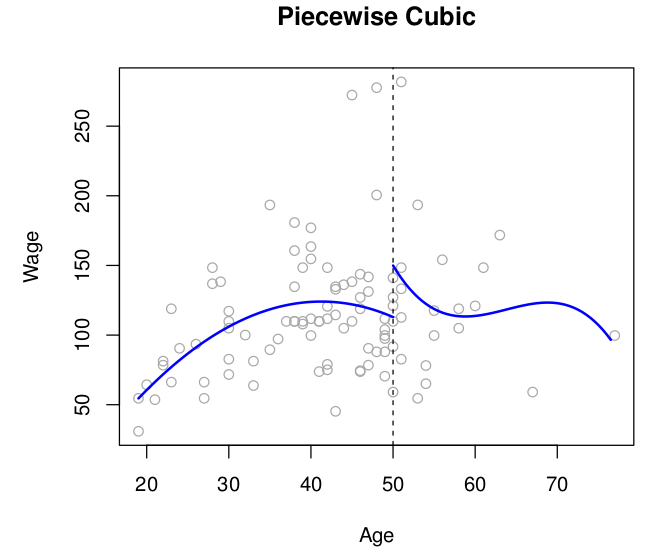
\includegraphics[width = \textwidth, align = c]{Fig7-3a}
\InstructorNotes{Piecewise cubic but discontinuous}
	
	\column{.3\textwidth}
	\centering
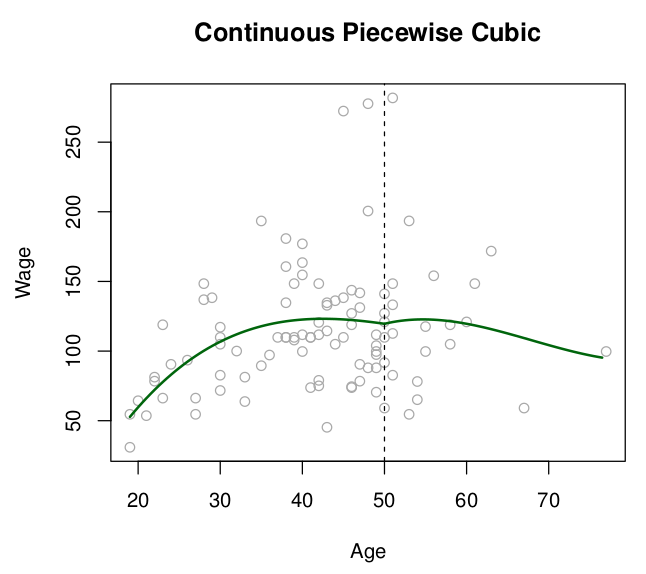
\includegraphics[width = \textwidth, align = c]{Fig7-3b}
\InstructorNotes{Continuous but pointy join}

	\column{.3\textwidth}
	\centering

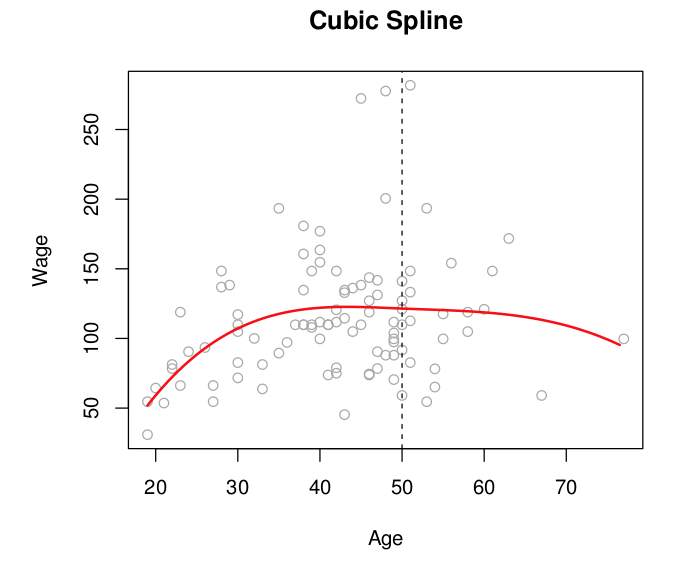
\includegraphics[width = \textwidth, align = c]{Fig7-3c}
\InstructorNotes{Smooth join. Same value plus same first and second derivatives.}
	\end{columns}
\bvfill 

	\centering
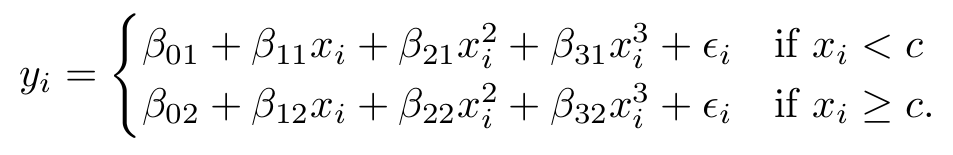
\includegraphics[width = .5\textwidth, align = c]{Eq7-8b.png}

Test your understanding: \href{https://PollEv.com/multiple_choice_polls/VfsOWK6ju6uRcPlbzliBJ/respond}{PollEv}
\end{frame}
%--- Next Frame ---%

%--- Next Frame ---%
\begin{frame}[t]{Cubic splines: degrees of freedom}

\begin{columns}
\column{.45\textwidth}
\centering
\begin{equation*}
	f(x) = 
	\begin{cases}
		\beta_0^1 + \beta_1^1 x + \beta_2^1 x^2 + \beta_3^1 x^3 & x<c \\
		\beta_0^2 + \beta_1^2 x + \beta_2^2 x^2 + \beta_3^2 x^3 & x>c
	\end{cases}
\end{equation*}

% \begin{itemize}
% 	\item Fit piecewise polynomial
% 	\item Require continuity at knots
% 	\item Require the first and second derivatives to be continuous at knots
% \end{itemize}
\InstructorList{
	\item 8 original degrees of freedom, plus three constraints (continuous, 1st deriv continuous, 2nd deriv continuous) leaves 5 degrees of freedom
	\item cubic spline with $K$ knots uses $4+K$ degrees of freedom
}
\column{.45\textwidth}
\centering
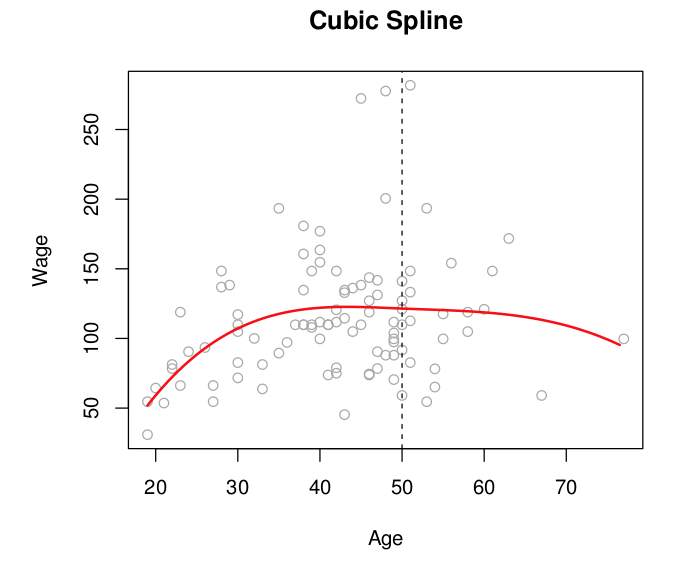
\includegraphics[width = \textwidth, align = c]{Fig7-3c}

\end{columns}

\end{frame}


%--- Next Frame ---%

\begin{frame}[t]{Notes on cubic splines }

\begin{columns}
\column{.45\textwidth}
\centering

\InstructorList{
  \item Human eyes can't detect the discontinuities so often cubic splines are a good way to go
	\item Still have problem of high variance at the outer range of predictors (big or small $X$)
	\item \textit{Natural spline:} regression spline plus boundary constraints where function is required to be linear at the boundary
}

\column{.45\textwidth}
\centering

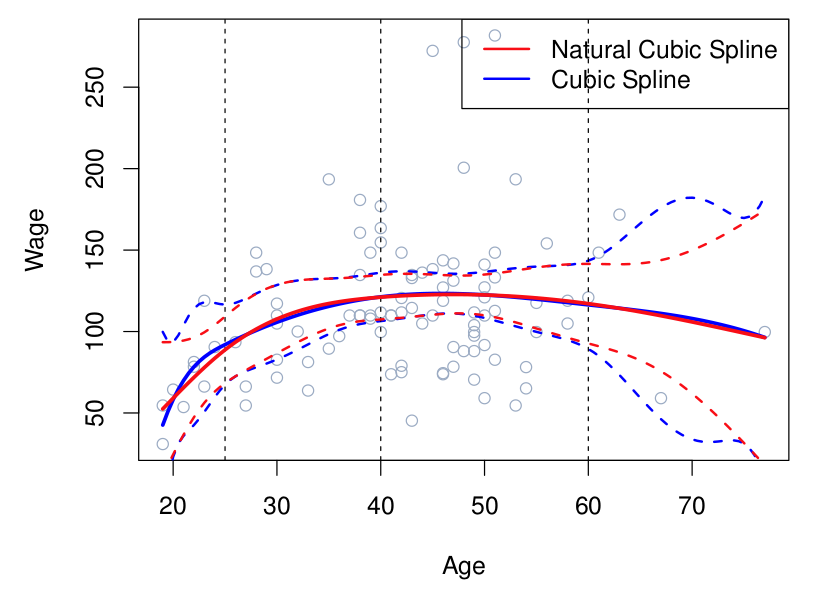
\includegraphics[width = \textwidth]{Fig7-4}
\end{columns}

\end{frame}
%--- Next Frame ---%
\begin{frame}[t]{Where to put the knots?}

\begin{columns}

\column{.65\textwidth}
\centering

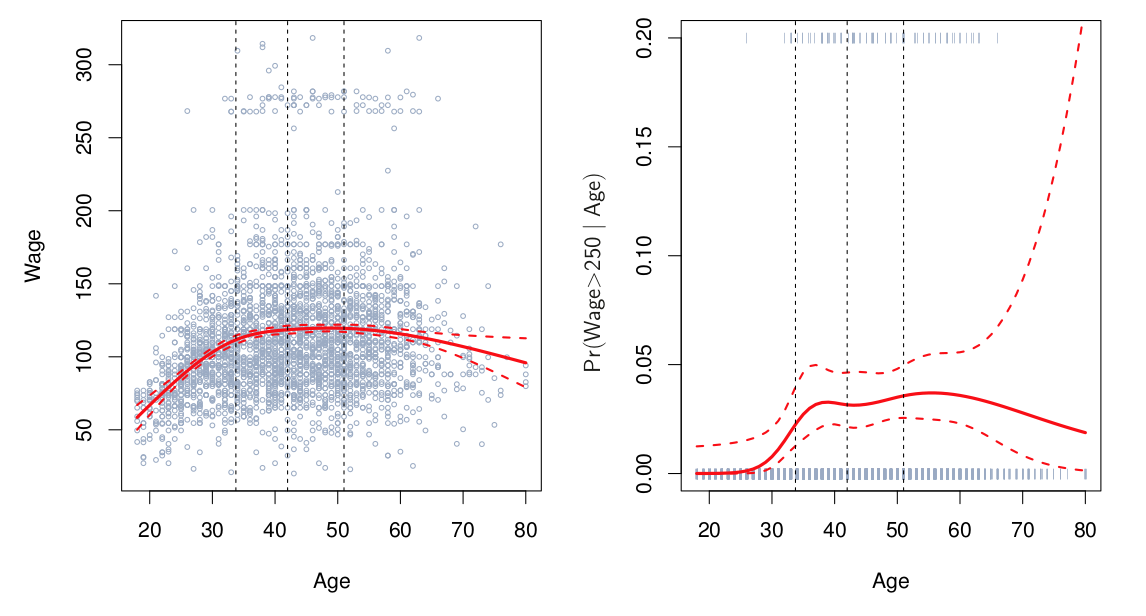
\includegraphics[width = \textwidth]{Fig7-5}
\column{.25\textwidth}
\centering

\InstructorList{
  \item Plan A: Uniform placement
	\item Plan B: Data driven. Example here puts it at quantiles of the data
}
\end{columns}

\end{frame}
%--- Next Frame ---%
\begin{frame}[t]{How many knots to use?}
{When in doubt, Cross-Validate.}
\begin{columns}
\column{.45\textwidth}
\centering

\InstructorList{
	\item need to know knot is a flexibility parameter, hence all the bias-variance trade-off stuff applies.
  \item Do CV ($k$-fold probably) on data for each number of knots
	\item Figure at right is the MSE resulting from 10-fold CV
	\item Note that clearly linear is not enough, after that 3-4 degrees of freedom for the cubic spline are enough
}

\column{.45\textwidth}
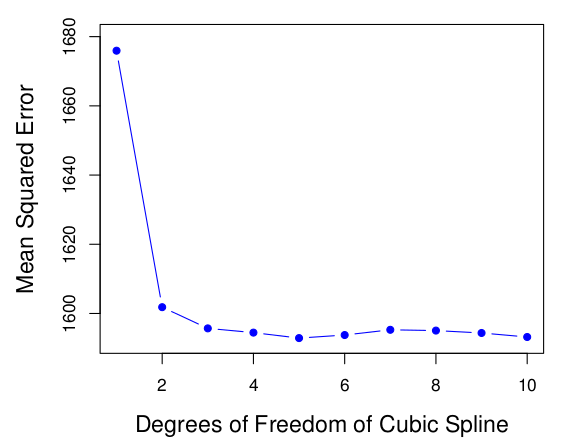
\includegraphics[width = \textwidth]{Fig7-6b}
\centering

\end{columns}
\end{frame}

%--- Next Frame ---%
\section{SVC vs SVM}
%--- Next Frame ---%

\begin{frame}[t]{Support Vector Classifier}

	\begin{columns}
	\column{.25\textwidth}
	\centering
	
	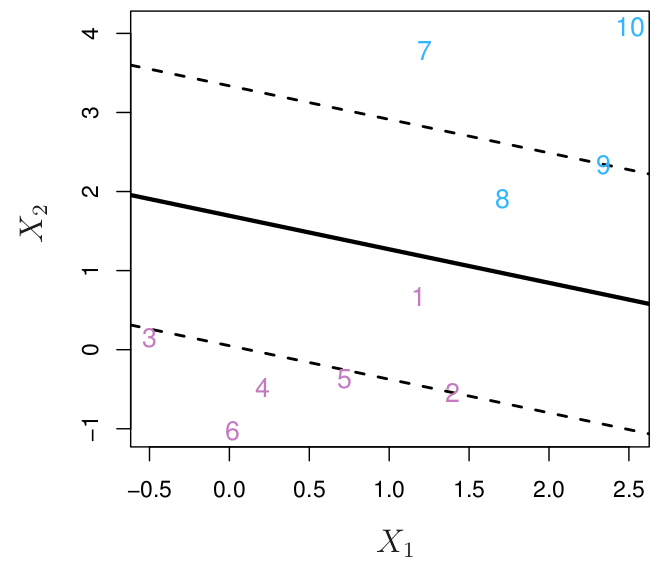
\includegraphics[width = \textwidth, align = c]{Fig9-6a}
	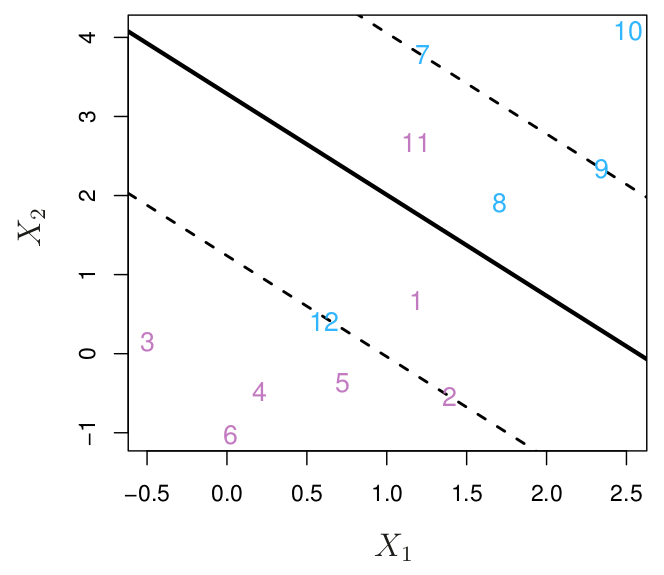
\includegraphics[width = \textwidth, align = c]{Fig9-6b}
	\column{.65\textwidth}
	\centering
	
	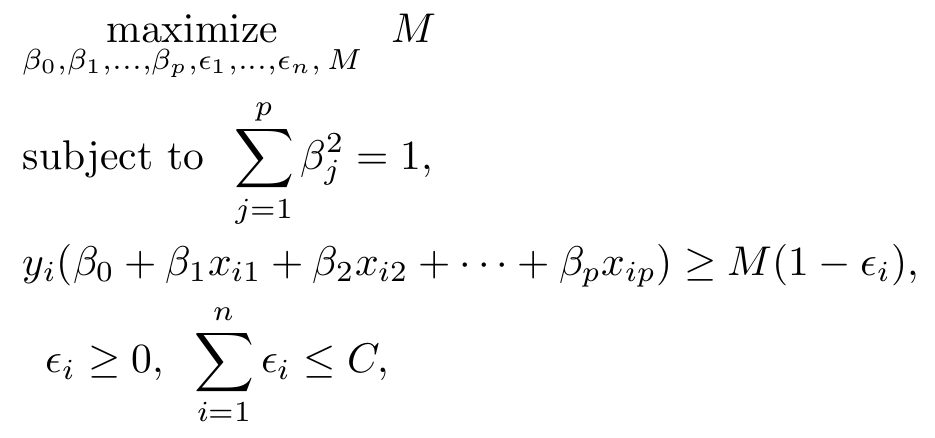
\includegraphics[width = \textwidth, align = c]{Eq9-12}
	
	\vspace{0.2in}
	
	\InstructorList{
	  \item Soft margin
		\item Allow for violations across margin
		\item Allow for violations across hyperplane
	}
	
	\end{columns}
	
\end{frame}
%--- Next Frame ---%
\begin{frame}[t]{So many variables}

	\begin{columns}
	\column{.45\textwidth}
	\centering
	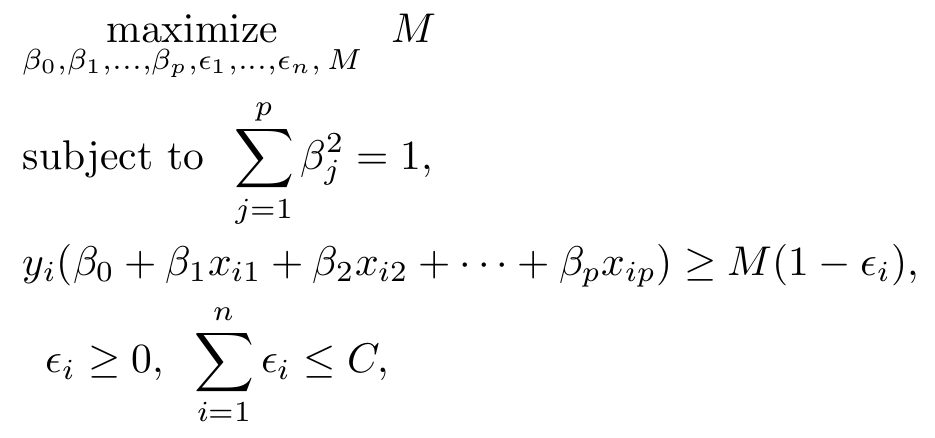
\includegraphics[width = \textwidth, align = c]{Eq9-12}
	
	\column{.5\textwidth}
	\centering
	\footnotesize
	\begin{itemize}
	  \item $C$ is nonnegative tuning parameter
	
		\InstructorList{
			\item Bounds sum of $\e_i$; number \& severity of violating margin (budget)
			\item $C=0$ means no violations allowed
			\item $C>0$ means at most $C$ observations can be on wrong side of hyperplane
			}
	
		\item $M$ is the width of the margin
		\item $\e_1, \cdots, \e_n$ are slack variables allowing observations to go to the other side
				\InstructorList{
			  \item If $\e_i = 0$, then on correct side of margin
				\item If $\e_i>0$ then on the wrong side of margin  (Violated margin)
				\item If $\e_i >1$ then on the wrong side of hyperplane
			}
	\end{itemize}
	
	\end{columns}
	
	\end{frame}

	
	\begin{frame}[t]{Limiting factor of SVC}
	
	\begin{columns}
	\column{.35\textwidth}
	\centering
	
	
	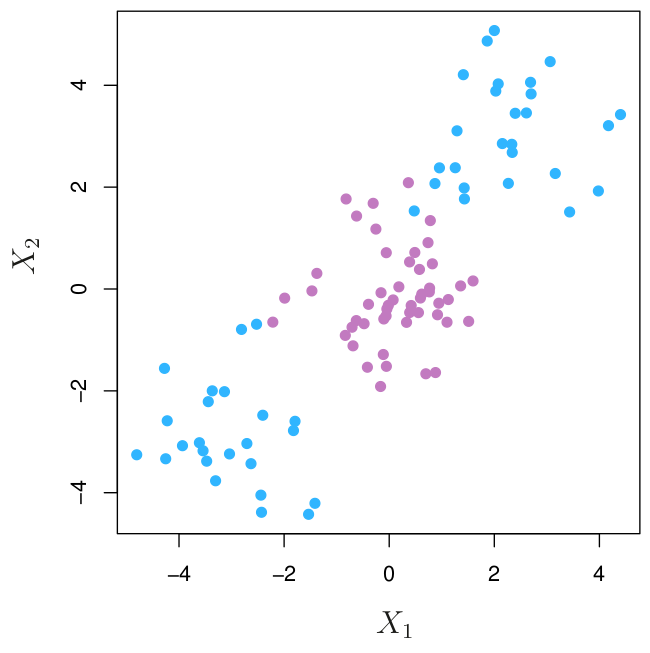
\includegraphics[width = \textwidth]{Fig9-8a}
	
	\column{.35\textwidth}
	\centering
	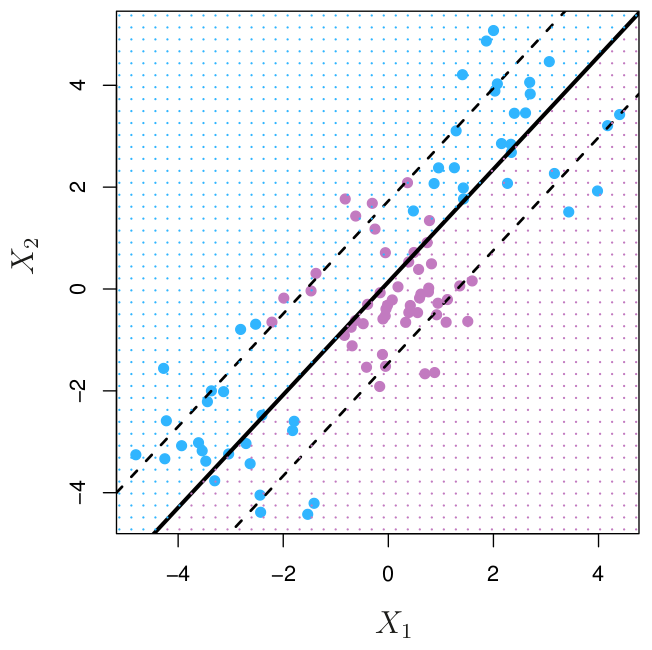
\includegraphics[width = \textwidth]{Fig9-8b}
	
	\end{columns}
	\InstructorList{
	  \item Requires linear boundaries
		\item "Non-linear" is a lot of things, how do you choose features to learn?
		\item Right side is result from SVC
	}
	\end{frame}

%--- Next Frame ---%

\begin{frame}[t]{More general way of thinking about constraints -- Kernels }

	\begin{columns}
	\column{.45\textwidth}
	\centering
	$y_i f(x_i)\geq M(1-\epsilon_i)$
	
	\InstructorList{
		\item Main idea: we can change up $f(x_i)$ to be nonlinear
		\item In fact, we do not need absolute coordinates of $x_i$. just need to know how close or similar to each other (draw points w/o coordinates)
		\item turns out just need to know general similarity between every two points - more computationally efficient
		\item Kernel: a more generalized way of thinking about how close or similar two samples are
		\item draw some examples in 1D
	}
	
	\column{.45\textwidth}
	$f(x_i)$ should give you some more general way of talking about how far is point $x_i$ away from the decision boundary.
	
	\InstructorList{
		\item alternatively, we can simply write $f(K(x_i, x1),K(x_i, x2),\cdots, K(x_i,x_p))$
		\item this is essentially in relative coordinates
	}
	\end{columns}
	
\end{frame}

\begin{frame}[t]{The kernel}

	\begin{columns}
	\column{.45\textwidth}
	\centering
	\begin{equation*}
		K(x_i,x_i')
	\end{equation*}
	\InstructorList{
	  \item Swap out my inner product $\langle x, x_i \rangle$ for something potentially more complicated
		\item $\langle x, x_i \rangle$ is known as a linear kernel
		% \item near kernel essentially quantifies the similarity of a
	% pair of observations using Pearson (standard) correlation
	}
	
	\column{.45\textwidth}
	\centering
	\begin{equation*}
		f(x) = \beta_0 + \sum_{i \in \mathcal{S}}\alpha_i K(x,x_i)
	\end{equation*}
	
	\InstructorList{
	  \item The function defined is as above with whatever choice of $K$
	  \item $K(x_i,x_i')$ can be thought of as similarity function.
		\item When the support vector classifier is combined with a non-linear kernel the resulting classifier is 	known as a support vector machine.
	}
	
	\end{columns}
	
	Test your understanding: \href{https://PollEv.com/ranking_polls/YdH5JVK2YdEhMm44VQu7S/respond}{PollEv}
	\end{frame}
	%--- Next Frame ---%
	\begin{frame}[t]{A polynomial kernel}
	\begin{equation*}
		K(x_i,x_{i'}) = \left(1 + \sum_{j=1}^p x_{ij}x_{i'j} \right)^d
	\end{equation*}
	\begin{columns}
	\column{.45\textwidth}
	\centering
	
	\InstructorList{
	  \item much more flexible decision boundary.
		\item amounts to fitting a support vector
	classifier in a higher-dimensional space involving polynomials of degree $ d$,
	rather than in the original feature space.
	\item Right: degree 3 polynomial kernel
	
	}
	
	\column{.35\textwidth}
	\centering
	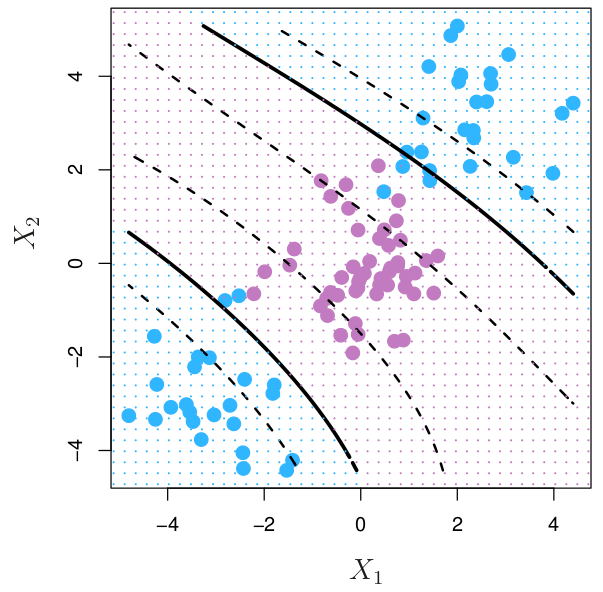
\includegraphics[width = \textwidth]{Fig9-9a}
	\end{columns}
	
	\end{frame}
	%--- Next Frame ---%
	
	
	\begin{frame}[t]{A radial kernel}
	\begin{equation*}
		K(x_i,x_i') = \exp \left( -\gamma \sum_{j=1}^p(x_{ij} - x_{i'j})^2 \right)
	\end{equation*}
	\begin{columns}
	\column{.45\textwidth}
	\centering
	
	\InstructorList{
	%   \item Draw picture of circular values around a point
	  \item this is essentially a gaussian kernel
		\item big distance makes $\sum (x_{ij}-x_{i'j})^2$ big, but then $e^{-big}$ is tiny.
		\item In $f(x)$, this means that $x_i$ plays little role if it's far away.
		\item Radial kernel has local behavior
	}
	
	\column{.35\textwidth}
	\centering
	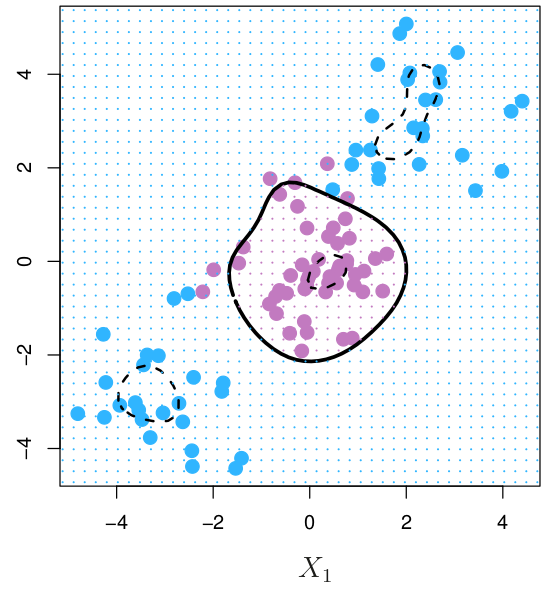
\includegraphics[width = \textwidth, align = c]{Fig9-9b}
	\end{columns}
	
\end{frame}

%--- Next Frame ---%


\begin{frame}[t]{TL;DR}

	\begin{columns}
	\column{.45\textwidth}
	\centering
	\begin{equation*}
		f(x) = \beta_0 + \sum_{i \in \mathcal{S}} \alpha_iK(x, x_i )
	\end{equation*}
	
	\column{.45\textwidth}
	\centering
	\footnotesize
	\textbf{Kernels}
	\begin{itemize}
		\item Linear
	\begin{equation*}
		K(x_i,x_{i'}) = \sum_{j=1}^p x_{ij}x_{i'j}
	\end{equation*}
		\item Polynomial
	\begin{equation*}
		K(x_i,x_{i'}) = \left(1 + \sum_{j=1}^p x_{ij}x_{i'j} \right)^d
	\end{equation*}
		\item Radial
	\begin{equation*}
		K(x_i,x_i') = \exp \left( -\gamma \sum_{j=1}^p(x_{ij} - x_{i'j})^2 \right)
	\end{equation*}
	\end{itemize}
	
	\end{columns}
	
\end{frame}

%==========
\section{Neural Nets}
%==========

%--- Next Frame ---%
\begin{frame}[t]{Feed Forward Neural Network: The cartoon}

\begin{columns}
\column{.45\textwidth}
\centering
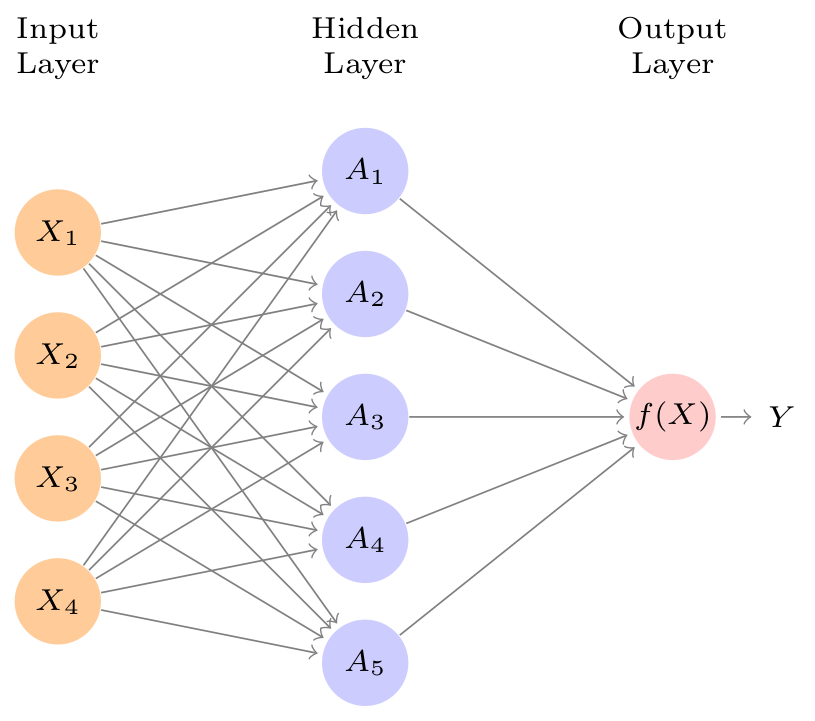
\includegraphics[width = \textwidth, align = c]{Fig10-1}
\column{.45\textwidth}
\centering
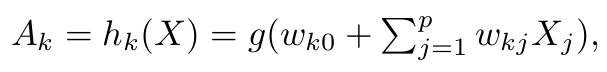
\includegraphics[align = c, width = \textwidth]{Eq10-2}
$\displaystyle{f(X) = \beta_0 + \sum_{k=1}^K \beta_k A_k}$

% Test your understanding: \href{https://PollEv.com/multiple_choice_polls/XuIKJuruOLR79NmpKJAqh/respond}{PollEv}

\InstructorList{
  \item Input layer is starting data
	\item Each arrow means taking combo of those values with weights to get next value
	\item Here there is one hidden layer then the output
	\item Get to pick how many hidden units $K$, here we have $K=5$
}

\end{columns}

\end{frame}
%--- Next Frame ---%

\begin{frame}[t]{Choices for activation function }

	\begin{columns}
	\column{.45\textwidth}
	\centering
	Sigmoid:
	\begin{equation*}
		g(z) = \frac{e^z}{1+e^z} = \frac{1}{1+e^{-z}}
	\end{equation*}
	% \InstructorList{
	%   \item Converts linear function in probabilities in [0,1]
	% }

	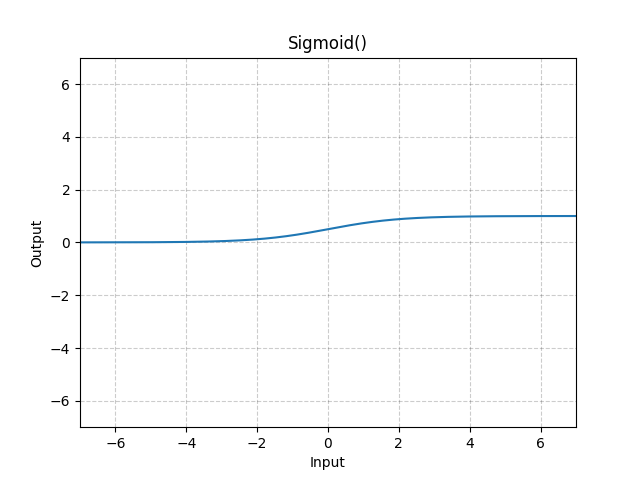
\includegraphics[align = c, width = \textwidth]{Sigmoid-pytorch}
	
	
	\column{.45\textwidth}
	\centering
	ReLU: Rectified linear unit
	\begin{equation*}
		g(z) = (z)_+ =
		\begin{cases}
			0 & \text{if }z<0 \\
			z & \text{else.}
		\end{cases}
	\end{equation*}
	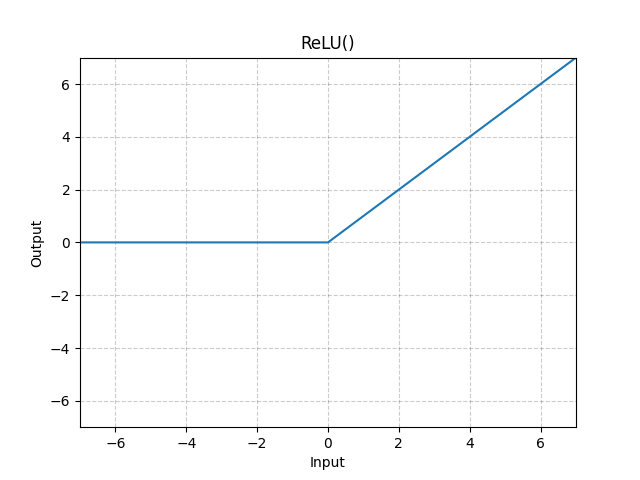
\includegraphics[align = c, width = \textwidth]{ReLU-pytorch}
	\end{columns}
	
	\end{frame}
	%--- Next Frame ---%
%--- Next Frame ---%



\begin{frame}[t]{Matrix version}
	\begin{columns}
	\column{.35\textwidth}
	\centering
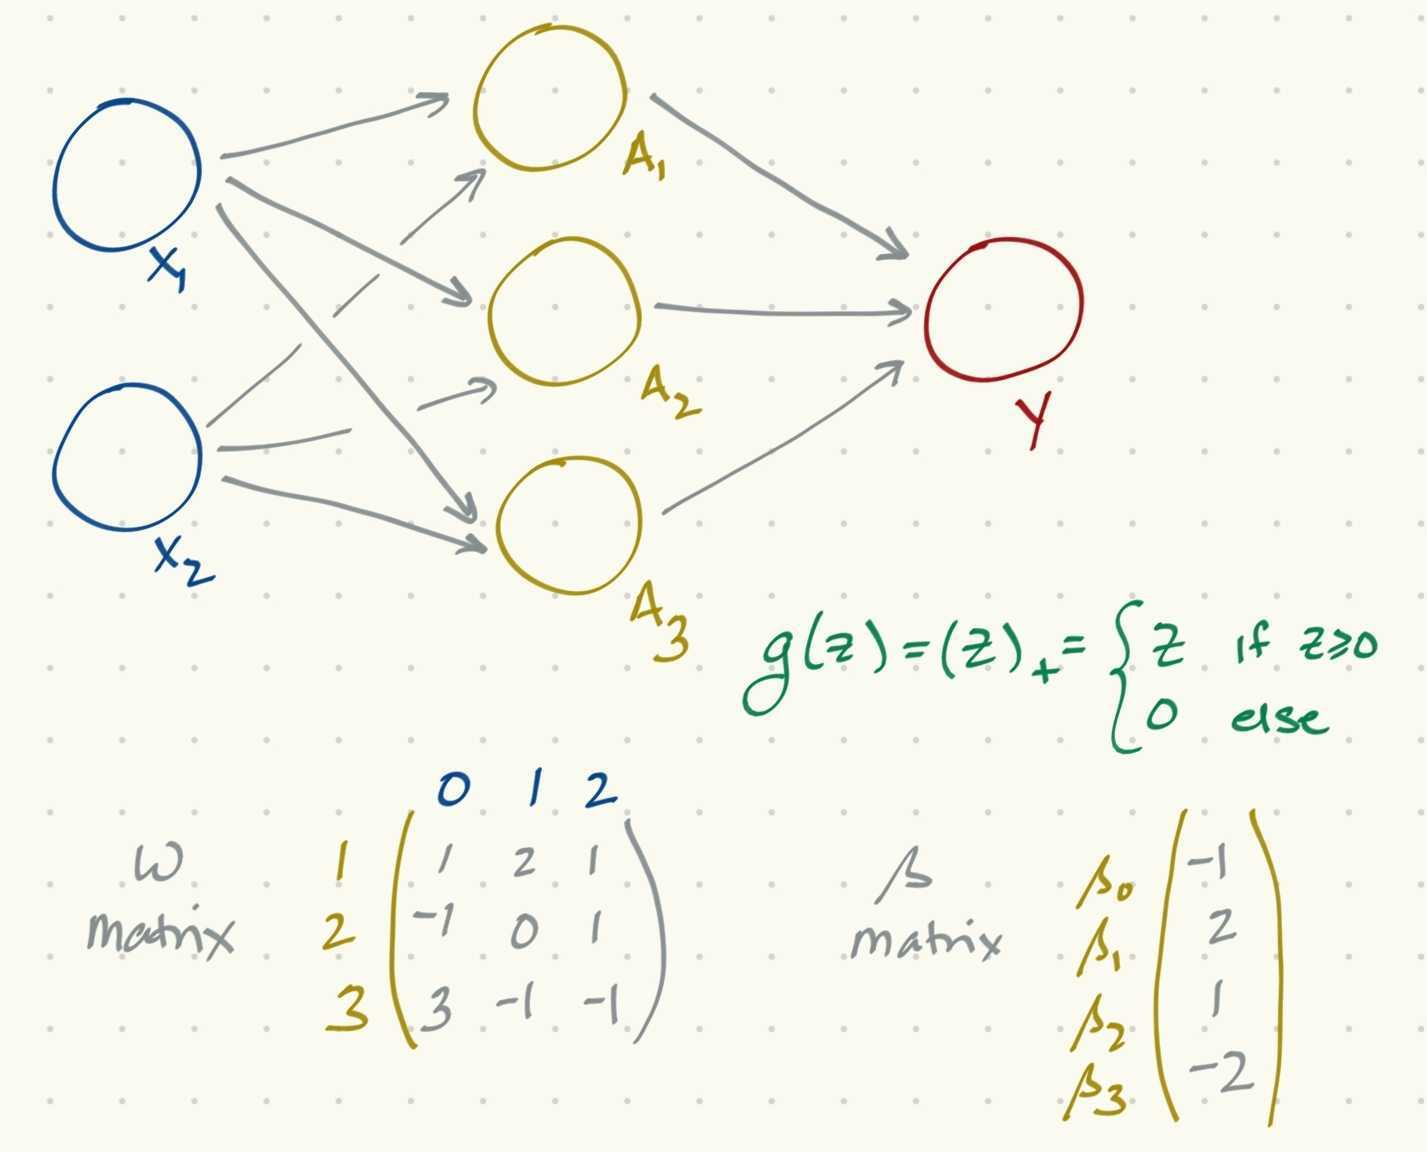
\includegraphics[width = \textwidth, align = c]{DL-simple-ex}
	
	\column{.55\textwidth}
	\centering
	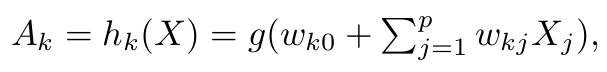
\includegraphics[width = .8\textwidth, align = c]{Eq10-2}
\begin{equation*}
	A = g( \mathbf{W}\cdot \mathbf{X})
	\qquad 
	\mathbf{X}^T = (1 \; X_1\; X_2\; \cdots \; X_p)
\end{equation*}

\vspace{.2in}

$\bowtie \bowtie \bowtie \bowtie \bowtie \bowtie $

\vspace{.2in}

$\displaystyle{f(X) = \beta_0 + \sum_{k=1}^K \beta_k A_k}$

\begin{equation*}
	Y = \beta \cdot \textbf{A}
	\qquad 
	\mathbf{A}^T = (1 \; A_1\; A_2\; \cdots \; A_K)
\end{equation*}
	\end{columns}
	\end{frame}
%-----------end frame------------

\end{document}
